\Chapter{Számítási teljesítmény mérése és összehasonlítása}

% Mért adatok demóhoz:
% WSL = [0.004772, 0.008008, 0.006689, 0.005726, 0.006113, 0.003458, 0.007568, 0.003998, 0.009867, 0.009790, 0.010321, 0.003363, 0.004423, 0.003769, 0.004492]
% Edge = [0.7999999998137355, 0.5, 1, 0.599999999627471, 0.6999999997206032, 0.6000000000931323, 0.6999999997206032, 0.7000000001862645, 1.099999999627471, 0.7000000001862645, 0.5999999940395355, 0.7000000029802322, 0.8999999910593033, 0.7000000029802322, 0.699999988079071]
% Firefox = [0.23999999999999488, 0.28000000000000114, 0.259999999999998, 0.35999999999999943, 0.3999999999999986, 0.259999999999998, 0.35999999999999943, 0.28000000000000114, 1.019999999999996, 0.28000000000000114, 0.259999999999998, 0.29999999999999716, 0.3200000000000003, 0.38000000000000256, 0.29999999999999716]
% Chrome = [0.7000000001862645, 1.3000000002793968, 1.2000000001862645, 0.8000000002793968, 0.7000000001862645, 0.7000000001862645, 0.599999999627471, 1.2000000001862645, 0.6999999997206032, 0.7999999998137355, 0.8999999910593033, 0.9000000059604645, 0.9000000059604645, 1.2000000029802322, 0.7000000029802322]
% VM = [0.001117, 0.003253, 0.004714, 0.002025, 0.001707, 0.001790, 0.000979, 0.004167, 0.002028, 0.001925, 0.001160, 0.001358, 0.002773, 0.001230, 0.001764]

% Mért adatok színátmenethez:
% Firefox = [11.04, 8.720000000000006, 10.520000000000003, 9.200000000000003, 8.240000000000002, 8.579999999999998, 7.48]
% WSL = [0.00356, 0.003790, 0.002984, 0.003454, 0.003536, 0.003269, 0.003308, 0.005547, 0.004861, 0.003949]

Az erőforrásigény összehasonlítását a Firefox egyik böngészőlapjának, és az én általam elkészített keretrendszerben egy példaalkalmazás memóriaigényét és CPU kihasználtságát egy Linux Mint virtuális gépben.

\Section{Mérés böngészőkben}

Először is a példa alkalmazást el készítettem egy HTML fájlként beágyazott Javascripttel. Miután biztosra mentem, hogy a két kód, ugyanazt az eredményt hozza grafikusan és a két ablak ugyanakkora, felhoztam a böngésző feladatkezelőjét. Az eredmény 511 KB memória és 0 CPU használat volt a böngészőlapnak. A futásideje a kódban lett mérve, amit tizenötször futattam, és \textit{Python} segítségével ábrázoltam.

A böngészők verziói pedig
\begin{itemize}
    \item Firefoxnak 100.0,
    \item Google Chrome-nak 101.0.4951.41,
    \item Microsoft Edge-nek 101.0.1210.32.
\end{itemize}

\subsection{Mérés demó programmal}

Továbbá, futtattam a kódot különböző böngészőkben a Windows 10-emben és a VM-ben is, amelynek a hisztogramja \aref{fig:hist-browsers}. ábrán látható. Az ábráról a láthatóság kedvéért ki lettek hagyva a böngészők VM-ben való futtatása, mert azok futásideje már [1,60] ms intervallumba esett. Ezekből az adatokból arra lehet következtetni, hogy az összes Chromium-alapú böngésző hasonló futásidővel fog futni, és hogy Firefox gyorsabb a Canvas API esetén, mint a Chromium-alapú böngészők.

A használt példa az alábbi forráskód és az eredmény \aref{fig:browser-canvas-example} ábra.

\begin{minted}{html}
<script>
    var canvas = document.getElementById("myCanvas");
    var ctx = canvas.getContext("2d");
    const start = performance.now();
    ctx.fillRect(0, 0, 100, 100);
    ctx.lineWidth = 20;
    ctx.strokeStyle = "#FF0000";
    ctx.strokeRect(50, 50, 100, 100);
    // Draw a blue triangle
    ctx.fillStyle = "#0000FF";
    ctx.lineWidth = 5;
    ctx.beginPath();
    ctx.moveTo(200, 200);
    ctx.lineTo(300, 200);
    ctx.lineTo(300, 300);
    ctx.closePath();
    ctx.fill();
    // Draw a green circle
    ctx.fillStyle = "#00FF00";
    ctx.lineWidth = 10;
    ctx.beginPath();
    ctx.arc(300, 500, 100, 0, Math.PI * 2, true);
    ctx.closePath();
    ctx.fill();
    // Write "Hello World"
    ctx.fillStyle = "#000000";
    ctx.lineWidth = 1;
    ctx.font = "24px Helvetica";
    ctx.fillText("Hello World", 500, 200);
    const duration = performance.now() - start;
    console.log("Time took: " + duration);
</script>
\end{minted}

\begin{figure}[h!]
    \centering
    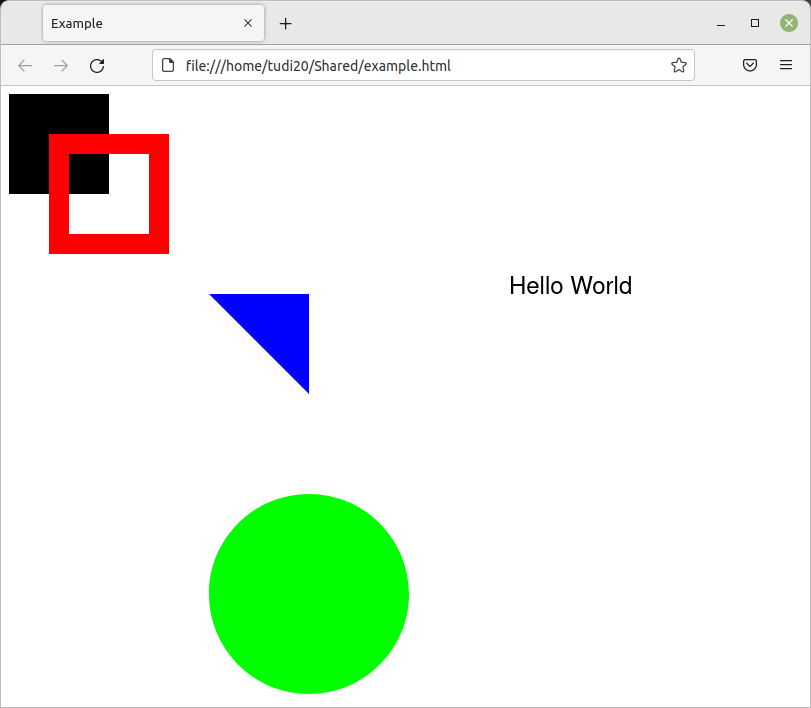
\includegraphics[width=8truecm]{images/browser_example.png}
    \caption{Böngészőben futatott példa eredménye}
    \label{fig:browser-canvas-example}
\end{figure}

\begin{figure}[h!]
    \centering
    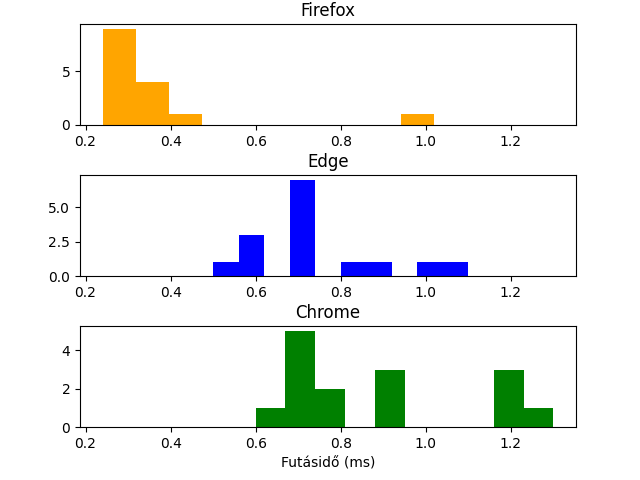
\includegraphics[width=14truecm]{images/histogram_browsers.png}
    \caption{Futásidő hisztogramja különböző böngészőkben}
    \label{fig:hist-browsers}
\end{figure}

\pagebreak

\subsection{Vonalhúzó méréssel}

Elkészült egy program is, ami 1280 alkalommal (a vizsgálathoz használt felbontás alapján) húz egy vonalat különböző színnel, így egy színátmenetet létrehozva. A létrehozott színátmenet \aref{fig:gradient}. ábrán látható. A kód ami létrehozta a színátmenetet pedig alább olvasható. Érdekes, hogy a színátmenet nem az, amire azonnal számítanánk a kódból.

\begin{minted}{javascript}
var canvas = document.getElementById("myCanvas");
var ctx = canvas.getContext("2d");
const start = performance.now();
ctx.strokeWidth = 2;
for (var i = 1; i < 1281; i++) {
    ctx.beginPath();
    ctx.moveTo(i - 1, (i - 1) % 2 ? 0 : 720);
    ctx.strokeStyle =
        "rgb(i / 1270.0 * 255,
        i / 1270.0 * 255,
        i / 1270.0 * 255)";
    ctx.lineTo(i, i % 2 ? 0 : 720);
    ctx.stroke();
}
const duration = performance.now() - start;
console.log("Time took: " + duration);
\end{minted}

\begin{figure}[h!]
    \centering
    
\includegraphics[width=8truecm]{images/gradient_native.png}
    \caption{Létrehozott színátmenet vonalhúzó méréssel}
    \label{fig:gradient}
\end{figure}

\pagebreak

\Section{Mérés az általam elkészített keretrendszerben}

A saját példaprogramomat lefordítottam és futtatam a háttérben majd felhoztam a rendszer figyelő alkalmazását. 104 KiB memória és 0 CPU használat mutatott. A HTML és JS kód megfelelője a keretrendszeremben az alábbi forráskód és az eredménye \aref{fig:own-example}. ábra.

\subsection{Demó programmal}

A futásidő is mérve lett a kódban hasonló módon -- a VM-ben és WSL-lel is -- majd hisztogramként \aref{fig:hist-own}. ábrán ábrzázolva is lett \textit{Python} segítségével.
\begin{minted}{c}
void draw(canvas_rendering_context_t* rendering_context)
{
    struct timespec start, end;
    clock_gettime(CLOCK_MONOTONIC, &start);
    canvas_fill_rectangle(rendering_context, 0, 0, 100, 100);
    canvas_set_line_width(rendering_context, 20);
    canvas_set_color(rendering_context, 255, 0, 0);
    canvas_stroke_rectangle(rendering_context, 50, 50, 100, 100);
    /* Draw a blue triangle */
    canvas_set_color(rendering_context, 0, 0, 255);
    canvas_set_line_width(rendering_context, 5);
    canvas_begin_path(rendering_context);
    canvas_move_to(rendering_context, 200, 200);
    canvas_line_to(rendering_context, 300, 200);
    canvas_line_to(rendering_context, 300, 300);
    canvas_close_path(rendering_context);
    canvas_fill(rendering_context);
    /* Draw a green circle */
    canvas_set_color(rendering_context, 0, 255, 0);
    canvas_set_line_width(rendering_context, 10);
    canvas_begin_path(rendering_context);
    canvas_arc(rendering_context, 300, 500, 100, 0, 360, 0);
    canvas_close_path(rendering_context);
    canvas_fill(rendering_context);
    /* Write Hello World */
    canvas_set_color(rendering_context, 0, 0, 0);
    canvas_set_line_width(rendering_context, 1);
    canvas_font2(rendering_context, "helvetica", 24);
    canvas_fill_text(rendering_context, "Hello World", 500, 200);
    clock_gettime(CLOCK_MONOTONIC, &end);
    printf("Time taken: %f\n", (end.tv_sec - start.tv_sec) +
    (end.tv_nsec - start.tv_nsec) / 1000000000.0);
}
\end{minted}

\begin{figure}[h!]
    \centering
    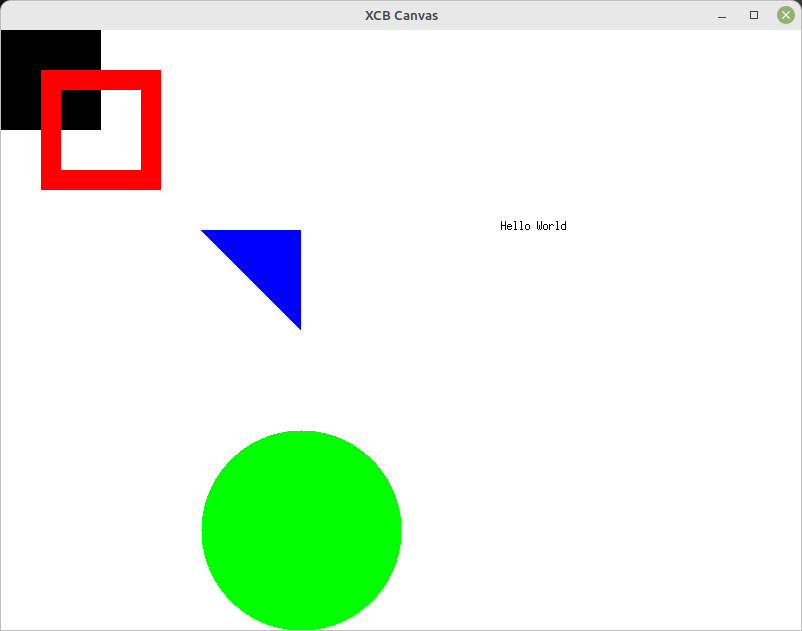
\includegraphics[width=8truecm]{images/own_example.png}
    \caption{Példa a saját keretrendszerben}
    \label{fig:own-example}
\end{figure}

\begin{figure}[h!]
    \centering
    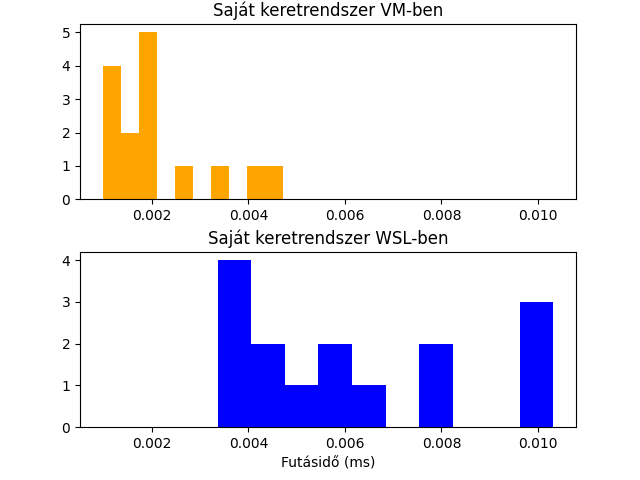
\includegraphics[width=14truecm]{images/histogram_native.png}
    \caption{Futásidő hisztogramja a saját keretrendszerben}
    \label{fig:hist-own}
\end{figure}

\subsection{Vonalhúzó méréssel}

A saját keretrendszerben is meg lett mérve az idő a vonalhúzó mérésben. A kódja hasonló módon készült el a fentihez. A keretrendszerem a böngésző esetében kapottal megegyező eredményt adott.

\begin{minted}{c}
struct timespec start, end;
xcbcanvas_set_window_size(rendering_context->canvas, 1280, 720);
clock_gettime(CLOCK_MONOTONIC, &start);
canvas_set_line_width(rendering_context, 2);
for (int i = 1; i < 1281; i++) {
    canvas_begin_path(rendering_context);
    canvas_move_to(rendering_context,
        (i - 1), (i - 1) % 2 ? 0 : 720);
    canvas_set_color(rendering_context,
        (int)(i / 1280.0 * 255),
        (int)(i / 1280.0 * 255),
        (int)(i / 1280.0 * 255));
    canvas_line_to(rendering_context, i, i % 2 ? 0 : 720);
    canvas_stroke(rendering_context);
}
clock_gettime(CLOCK_MONOTONIC, &end);
printf("Time taken: %f\n", (end.tv_sec - start.tv_sec) +
(end.tv_nsec - start.tv_nsec) / 1000000000.0);
\end{minted}

\pagebreak

\Section{Összehasonlítás}

A keretrendszerem csak a Canvas API primitívek rajzolását, Path rajzolását görbék nélkül, és a szöveg írásának minimális lehetőségét fedi le, és a memóriának csak a 20\%-át használja. Ellentétben viszont, a keretrendszeremben lassabban lehet tesztelni, hogy helyes kódot írtunk, ugyanis a gépi kódra fordítás lassabb, mint egy böngészőben betölteni egy helyi weboldalt. Továbbá össze akartam hasonlítani a már létező xcb-canvas-val, de nem sikerült a használata.

\subsection{Demó programnál}

A futási időt tekintve a keretrendszerem ~0.28 ms-ről ~0.007 ms-re csökkent, azaz negyvenszer lett gyorsabb.
Az ezt összehasonlító hisztogram látható \aref{fig:hist-compare}. ábrán.

\begin{figure}[h!]
    \centering
    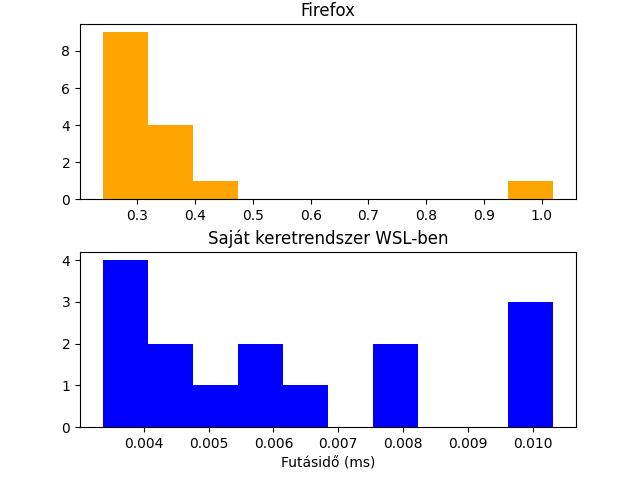
\includegraphics[width=14truecm]{images/histogram_compare.png}
    \caption{Futásidőt összehasonlító hisztogram. Míg Firefox 0.2 ms alá nem esik, addig WSL 0.01 ms-nél csak gyorsabb szokott lenni.}
    \label{fig:hist-compare}
\end{figure}

\subsection{Vonalhúzó mérésnél}

A mérés ebben az esetben csak Firefoxban és WSL-ben történt tízszer. Ha ezt a mérés vesszük figyelembe akkor a WSL 2558-szor gyorsabb, mint Firefox. Ezeknek a mérésneknek a hisztogramjai \aref{fig:hist-compare-gradient}. ábrán tekinthető meg.

\begin{figure}[h!]
    \centering
    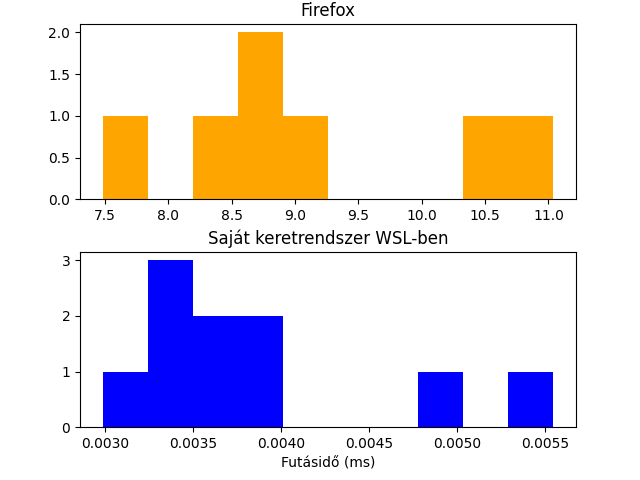
\includegraphics[width=14truecm]{images/histogram_compare_gradient.png}
    \caption{Futásidőt összehasonlító hisztogram a vonalhúzó mérés alkalmazásban.}
    \label{fig:hist-compare-gradient}
\end{figure}